% \chapter{Background}
In this chapter, we provide some insight into the different technical concepts, which need to be understood in order to comprehend the design decisions we make in this thesis. We will first discuss the MONDRIAN network zoning architecture, followed by some characteristic features regarding data center networking, then we will discuss \acl{SDN} and finally \acl{NFV}. 

\subsection{MONDRIAN}\label{sec:MONDRIAN}
\subsubsection{Overview}
MONDRIAN is an inter-domain network zoning architecture, which has been proposed in a paper \cite{kwonmondrian} written by researchers at \acs{ETH} Zurich (\acl{ETH} Zurich). In large networks, assets with similar security requirements are typically grouped together into subnets. Transitions from one subnet into a different one need to be allowed by configuring one or multiple routers accordingly. This process is cumbersome, prone to errors and especially hard to realize in an inter-domain scenario.

MONDRIAN tackles this problem by making two major abstractions. Firstly, it introduces the concept of networking zones, which typically consist of one or more subnets, which can be located at geographically distributed sites. Zones group together assets with similar security requirements across sites. Secondly, MONDRIAN logically centralizes the management of zone transitions by introducing a MONDRIAN Controller, which hosts a policy database, which allows for easy administration of transition policies on a zone level. The transition policies are checked and enforced by \aclp{TP}, of which there exists one per site. The placement of the \acsp{TP} (\aclp{TP}) and the MONDRIAN Controller is shown in figure \ref{MONDRIAN Overview}.  

\begin{figure}[t]
	\centering
	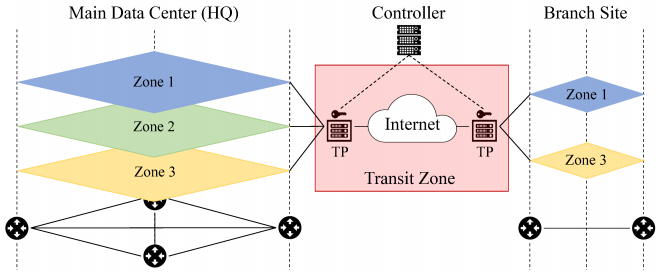
\includegraphics[width =0.48\textwidth]{img/mondrian_overview.png}
	\caption{MONDRIAN Overview\cite{kwonmondrian}}
	\label{MONDRIAN Overview}
\end{figure}

%\todo{\\
%    - What is MONDRIAN used for\\
%    - What does it replace\\
%    - What are zones/zone-transitions\\
%    - Show placement of TPs and MONDRIAN Controller
%}
\subsubsection{MONDRIAN Controller}
A MONDRIAN Controller is the brain of a MONDRIAN deployment. It hosts the databases containing all the information that is used by the \acsp{TP}, including the zone transition policies. Therefore, it needs to be reachable by the \acsp{TP} and is typically exposed to the Internet. Even though for redundancy reasons there might be multiple instances of a MONDRIAN Controller, all of them need to be synchronized. This means that logically there is just one MONDRIAN Controller. Furthermore, a MONDRIAN Controller exposes a \acs{REST}ful \acs{API} (\acl{API}), which allows an administrator to update the data which is stored on the MONDRIAN Controller. 

%\todo{\\
%    - Explain what a MONDRIAN Controller is used for\\
%    - Controller logically centralizes the management of zone transition policies
%}
\subsubsection{Translation Point}
A \acl{TP} has two main responsibilities. It needs to check the authorization of zone transitions according to the zone transition policies and it provides an \acs{IP}-tunneling functionality, comparable to a \acs{VPN}. The construction of a \acs{TP} is very modular. It consists of three modules. The \textbf{Core Module} is responsible for simple parsing and packet handling activities. The \textbf{Transition Module's} responsibility is zone transition authorization and the \textbf{Authentication Module} provides the tunneling mechanism.

%\todo{\\
%    - One TP per site\\
%    - transition authorization\\
%    - IP-tunneling
%}
\paragraph{Transition Module}
The Transition Module checks packets against policies of the form shown in formula \ref{policy}. Note that since we are using zone-IDs, the policies are independent of site or subnet specific information. If the 5-tuplet matches a packet, the $action$ takes effect. Possible actions are $forwarding$, $drop$ and $established$, which are comparable to actions found in \texttt{iptables}, but with a zone level granularity. The attribute $proto$ signifies the transport layer protocol. Currently \acs{TCP} (\acl{TCP}) and \acs{UDP} (\acl{UDP}) are supported. All of the fields in the 5-tuplet can also be wildcards, which means that the zone-ID, port or protocol can be arbitrary. 
\begin{equation}\label{policy}
    <zoneID_{dst}, port_{dst}, zoneID_{src}, port_{src}, proto>\Rightarrow <action>
\end{equation}
%\todo{Authorize zone transitions based on policies (5-tuplets,  action)}    

\paragraph{Authentication Module}
The Authentication Module is responsible for guaranteeing confidentiality, authenticity and end-host anonymity of packets, which traverse the untrusted Internet or \acs{WAN} (\acl{WAN}). It achieves that by encrypting the original \acs{IP} (\acl{IP})-packet and passing it together with an authentication token into a MONDRIAN-packet, which is basically an additional \acs{IP}-layer with an authentication token as metadata and the encrypted \acs{IP}-packet as payload. The authentication token consists of a type identifier, the destination's zone-ID, a timestamp, a nonce as well as a \acs{MAC} (\acl{MAC}). To perform the authentication as well as the encryption/decryption, MONDRIAN uses symmetric cryptography with keys that can be dynamically derived according to the \acs{DRKey} (\acl{DRKey}) \cite{perrig2017opt} derivation scheme. The derived keys provide authenticity on a site-to-zone level granularity, which means that the derived key depends on the site of the sender and on both the site as well as the zone of the destination.

%\todo{\\
%    - Create MONDRIAN packet\\
%    - IP-tunneling site-to-zone level\\
%    - protect confidentiality \& integrity of inter-domain traffic
%}

\subsection{Data Center Networking}\label{Data Center Networking}
Networking in data centers is different in many ways from networking in corporate networks or \acs{Telco} (\acl{Telco}) networks. Topologies are much more standardized and specialized, most of the infrastructure is virtualized and performance is essential.

%\todo{Highlight difference between networking in corporate networks (north-south vs east-west traffic)}
\subsubsection{Topology}
Network topologies in data centers are highly optimized for the kind of traffic they need to be able to handle and the desired properties or assurances the use case requires. These properties can range from minimal latency between hosts to bandwidth guarantees and congestion prevention. Mostly however, it boils down to saving costs while having the performance that is required by the application. While there exist many experimental topologies like Fat-tree \cite{LeisersonFatTree}, Jelly Fish \cite{singla2012jellyfish}, DCell \cite{guo2008dcell} or BCube \cite{guo2009bcube} to name a few, most of the topologies are a variation of the Leaf-Spine topology, where scalability is often achieved by using clos networks to replace switches with too few ports. Typically, data center topologies are built up using a three-tier layout consisting of a core layer, an aggregation layer and an access layer.
%\todo{\\
%    - Specialized for the traffic that it needs to handle\\
%    - hierarchical setup\\
%    - leave-spine, clos, etc.\\
%    - experimental topologies --> flexibility needed
%}
\subsubsection{Virtualization}
In data centers we have an extremely high degree of virtualization. End-hosts are usually \acsp{VM}, containers or entire Kubernetes clusters. However, not only end-hosts are virtualized. Many of the network functions like learning switches, routers, load balancers or even firewalls are virtualized into \acsp{VNF} (\aclp{VNF}). \acl{NFV} has traditionally been realized by simply deploying a \acs{VM}, which implements the desired functionality. With the gaining popularity of \acs{SDN}, more and more \acsp{VNF} (\aclp{VNF}) are implemented as an application running on top of an \acs{SDN} controller. Usually, the switch a host is directly connected to is the virtual switch, which is a part of the hypervisor and connects the VMs to each other and to the rest of the network. These virtual switches are often based on the \acs{OVS} (\acl{OVS}), which is a virtual switch that integrates well with OpenFlow, the de facto standard southbound \acs{SDN} protocol.

%\todo{\\
%    - Hosts = VMs, Containers\\
%    - network functions are often virtualized\\
%    - Hypervisors connect VMs via virtual switches to the rest of the network (mostly using OVS)
%}
\subsubsection{Performance}
In data centers, the computing resources are heavily monetized. A decrease in performance therefore results in immediate money loss. Many applications in data centers require the close collaboration between multiple hosts. Meaning that there's a lot of communication happening between hosts within the same data center. Consequently,  the performance bottleneck many applications experience lies in the network, which results in extremely high performance requirements for \acsp{VNF}, especially for \acsp{VNF} that affect east-west traffic, which makes up about 80\% of all network traffic in a typical data center \cite{talpurnetwork}. Data center networks are highly specialized for this kind of east-west traffic. Traffic engineers make sure that the strict performance requirements are met. It is therefore paramount that a new \acs{VNF} does not divert traffic from the originally intended route unless it's absolutely necessary.

%\todo{\\
%    - Performance is important\\
%    - bad performance = loss of money\\
%    - east-west performance is the most important 80\% \\ 
%    - DC networks are highly optimized for performance\\
%    - Don't divert traffic from original route
%}
\subsection{Software Defined Networking}
Networks based on \acs{SDN} are built up in three layers. The Infrastructure Layer consists of \acs{SDN} switches, which are controlled by an \acs{SDN} controller, which is located in the Control Layer. The topmost layer is the Application Layer, which is where business applications reside \cite{braun2014software}. The communication between the Infrastructure Layer and the Control Layer happens using a southbound protocol. The de facto standard for southbound \acs{SDN} protocols is called OpenFlow \cite{braun2014software}. While it's not the only southbound protocol, it is by far the most prominent one. As an interface between the Control Layer and the Application Layer, we have northbound interfaces. Since these interfaces are specific to the \acs{SDN} controller they are based on, there exists no standard for northbound interfaces. Some of the more popular \acs{SDN} controllers are Floodlight, HP VAN, POX, NOX or RYU \cite{tijare2016northbound}. Each of them has its own northbound \acs{API}. Some of the northbound interfaces are \acs{REST}ful \acsp{API}, which are usually used when a proactive strategy is employed, meaning that flow table entries are statically installed on the \acs{SDN} switches. If we employ a reactive strategy, meaning that we react to packets being sent to the \acs{SDN} controller via a packet-in message, then \acs{REST}ful \acsp{API} are not sufficient and we need a non-\acs{REST}ful \acs{API}. 
%\todo{\\
%    - Controller controlling switches\\
%    - Southbound protocol: OpenFlow = defacto standard\\
%    - Northbound API: No defacto standard \\
%    - Proactive vs. Reactive approach
%}
\subsection{Network Function Virtualization}
Virtualizing network functions has many benefits. It increases scalability, flexibility and resiliency. New networking components can be created and destroyed dynamically, without the need to move around physical hardware. This means that entirely new topologies can be created and reconfigured on the go, making it possible to meet different requirements at different points in time. Such a high degree of flexibility is needed in large data centers, where \acsp{VM} can be moved around and where traffic patterns can change instantly. While \acsp{VNF} are relatively new, there are already efforts to standardize \acs{NFV}. This process is mainly advanced by an organization called \acs{ETSI} (\acl{ETSI}).

Traditionally, \acsp{VNF} have been implemented on top of \acsp{VM}. This approach has the advantage that the \acsp{VNF} can perform any task that the underlying hardware is capable of handling. The major disadvantage is that \acsp{VM} can be quite resource consuming and take a relatively long time to spin up and down. Furthermore, \acsp{VM} require general purpose hardware, meaning that such \acsp{VNF} can't easily take advantage of specialized hardware like the one that can be found in switches. With the raising popularity and increasing maturity of \acs{SDN}, developers started implementing network functions as \acs{SDN} business applications. This has the advantage that some of the workload can be offloaded to the switches, where it's handled more efficiently and faster. However, not everything can be offloaded to \acs{SDN} switches. Computationally expensive operations like encryption and decryption can't be performed by switches. Since switches need to be very fast, they only support simple matching operations and can make forwarding decisions based on these matches.

%\todo{\\
%    - Standardization of NFV  \\
%    - Classical NFV based on VMs/Containers \\
%    - NFV based on SDN (Benefits, limitations)
%}

%\subsection{Related Work}
%The most important paper related to this thesis is of course the original MONDRIAN paper, proposing the original design of MONDRIAN \cite{kwonmondrian}. 
%
%What modern data centers look like and what concepts exist in the field of \ac{SDDC} is discussed in a whitepaper about VMware\texttrademark's NSX data center platform \cite{vmware2021nsx}. Current research questions concerning cloud data centers and where in data centers high costs occur and what the challenges are to minimize them is discussed in the paper \textit{The Cost of a Cloud: Research Problems in data center Networks} \cite{greenberg2008cost}.
%
%Regarding \ac{SDN}, there is a paper written by Intel\texttrademark,  discussing how a \ac{DPDK} enabled \ac{OVS} can enable \ac{SDN} and \ac{NFV} transformation \cite{intel2015OVS}. A great overview over the numerous northbound interfaces that exist for \ac{SDN} is provided by a paper called \textit{The Northbound APIs of Software Defined Networks} \cite{tijare2016northbound}. For gaining a basic understanding of the overall concepts of \ac{SDN}, I can recommend the book \textit{Software Defined Networks} by Paul Goransson and Chuck Black \cite{goransson2014SDN}.
%
%In the field of \ac{NFV} there exist a paper highlighting the benefits, enablers and challenges for \ac{NFV} \cite{att2012NFV}. This paper is a collaborative work of many major \ac{Telco} companies and has been presented at the \textit{\ac{SDN} and OpenFlow World Congress}.



%\todo{ \\
%	- original mondrian paper \cite{kwonmondrian}\\
%	- what DCs look like \cite{vmware2021nsx}\\
%	- what is important in DCs \cite{greenberg2008cost}\\
%	- OVS for SDN based NFV with DPDK \cite{intel2015OVS}\\
%	- Northbound APIs \cite{tijare2016northbound}\\
%	- Basics about SDN \cite{goransson2014SDN}\\
%	- NFV \cite{att2012NFV}
%}